
\chapter{Research Protocol}

\vcomment{List all decisions you make. Be very explicit.
	Current plan: Go into depth for certain portions in the implementations chapter.}

\section{Samples / Image Domain}\label{sec:NCS-data-set}

% see Nen's master's thesis for his descriptions of the data sets

We ultimately perform a PCSVN extraction on a set of 174 color placental images from a private database called NCS (from NYMH?). These are project files in GIMP which contain multiple layers.
The layers together give a hand tracing of the vascular network and perimeter. A sample of overlaid layers in a representative sample is given in \cref{fig:exampleNCSoutput}

\begin{figure}[h]\label{fig:NCSlayers} \centering
	\subfloat[Fixed Placental Sample]{
		\label{fig:NCSlayers-raw}\includegraphics[width=60mm]{{{T-BN0164923.raw}}}
		}
	\subfloat[Arterial tracing]{
		\label{fig:NCSlayers-A}\includegraphics[width=60mm]{{{T-BN0164923_arteryoverlay}}}
		}
	\subfloat[Venous tracing]{
		\label{fig:NCSlayers-V}\includegraphics[width=60mm]{{{T-BN0164923_veinoverlay}}}
		}
	\subfloat[Total Vascular Network]{
		\label{fig:NCSlayers-T}\includegraphics[width=60mm]{{{T-BN0164923_traceoverlay}}}
		}
\caption{A representative placental NCS sample with vascular tracing}
\end{figure}

In \cref{fig:NCSlayers-raw}, a cleaned, fixed placenta is shown. A detailed description of this procedure is given in \vtodo{some reference}. \cref{fig:NCSlayers-A} and \cref{fig:NCSlayers-V} are both hand traces of the PCSVN, with a layer for each the arteries and veins. In our particular use case, there is no need to consider them separately, so we simply consider them together, as in \cref{fig:NCSlayers-T}. The coloration is meant to indicate the diameter of each vessel. There is also a cord insertion point notated, as well as the perimeter of the placental plate.  These are hand-traced and rather labor intensive. A closer look at many of the samples often reveals some subjectivity in the tracings (often it's hard to see where the vein is, vascular networks are obscured, etc.) 



\begin{figure}\label{fig:exampleNCSoutput} 	\centering
	\subfloat[Background Mask]{
		\label{fig:NCSoutput-mask}\includegraphics[width=60mm]{{{T-BN0164923.mask}}}
		}
	\subfloat[Sample with BG removed]{
		\label{fig:NCSoutput-base}\includegraphics[width=60mm]{{{T-BN0164923}}}
		}
	\subfloat[Grayscale]{
		\label{fig:NCSoutput-gray}\includegraphics[width=60mm]{{{T-BN0164923.L}}}
		}
	\subfloat[Trace / ``Ground Truth'']{
		\label{fig:NCSoutput-trace}\includegraphics[width=60mm]{{{T-BN0164923.trace}}}
		}
	\caption{Preprocessed files from an NCS sample}
\end{figure}

For our procedure, we simply operate on the placental sample itself, without any understanding of its provided tracing except for comparing the strength of our algorithm. Of course, our goal is to develop an algorithm that can produce a ``ground truth'' tracing such as in \cref{fig:NCSlayers-T} or \cref{fig:NCSoutput-trace} without any intervention.

For our purposes however, we will use the provided placental perimeter (shown in green in \cref{fig:NCSlayers}. In developing a fully automated algorithm, it would be relatively straightforward to obtain this boundary ourselves using an Active Contour Model \vtodo{REF} or perhaps even any edge finding algorithm followed by morphological / watershedding as in \vtodo{REF}.



To build a sample suitable for use in our algorithm from \cref{fig:NCSlayers} is relatively simple. We "zero" outside the boundary of the plate (so as to not waste computational time calculating the differential geometry of a ruler, say), and also generate a binary mask to identify the plate. Finally, our vessel layers are combined and given as a binary trace.

These procedures are performed automatically on the 174 image in our data set using a custom GIMP plug-in, which performs various ``bucket fill'' operations, layer mergings, and thresholdings. For completeness sake, this plug-in (and an associated Scheme script which turns it into a batch operation) can be found in the Appendix. \vtodo{put a link here}
(There are actually 201 images but 27 of them have mislabeled layers and were not autoprocessed correctly)


\section{Image Preprocessing}
	
	As a point of technicality, the grayscale image in \cref{fig:NCSoutput-gray} is not actually produced directly by the extractor plug-in, but created when the 3 channel RGB image \cref{fig:NCSoutput-base} is imported at the start of the algorithm. This grayscale conversion is simply done for ease of analysis on the sample: although the Frangi filter is designed for arbitrary dimension input \cite{frangi1998multiscale}, an image with three color channels does not have 3 spatial dimensions. We therefore simply combine the information in three channels using the well-known and oft-implemented ITU-R 601-2 luma \cite{scipy}, or ``luminance'' transform:
	
	\begin{equation} \label{eq:luma_transform}
	L =  \frac{299}{1000}\ R + \frac{587}{1000}\ G + \frac{114}{1000}\ B
	\end{equation}

`	All images are grayscale, $M,N$ pixels as a masked array (of type
	\texttt{numpy.ma.MaskedArray}), where pixels outside of the placental region are masked so they will not be considered by the algorithm. However, some standard
	implementations of algorithms, namely \texttt{numpy.gradient and scipy.signal.convolve2d} are not designed to handle masked regions. Although it would be of some interest to create an algorithm that, say, calculates a gradient or performs a convolution by a ``reflection'' across an arbitrary closed boundary (as opposed to the edge of the image matrix), we opted instead to simply exclude affected areas from consideration, and zero unwanted background pixels to speed up computation. This excluding function,
	\texttt{plate\_morphology.dilate\_plate}, ultimately relies on two functions
	provided by the Python library \texttt{scikit-image} \cite{skimage}. The first, \texttt{skimage.segmentation.find\_boundaries()}, takes the mask input (such as \cref{fig:NCSoutput-mask}) and calculates where differences in a morphological erosion and dilation occur. That boundary itself is then dilated by the desired factor. The second is a ``sparse'' implementation of binary dilation that is particularly efficient for our problem. An array of indices of the image where the 
	
	\begin{figure}  \label{fig:boundary-demo}
		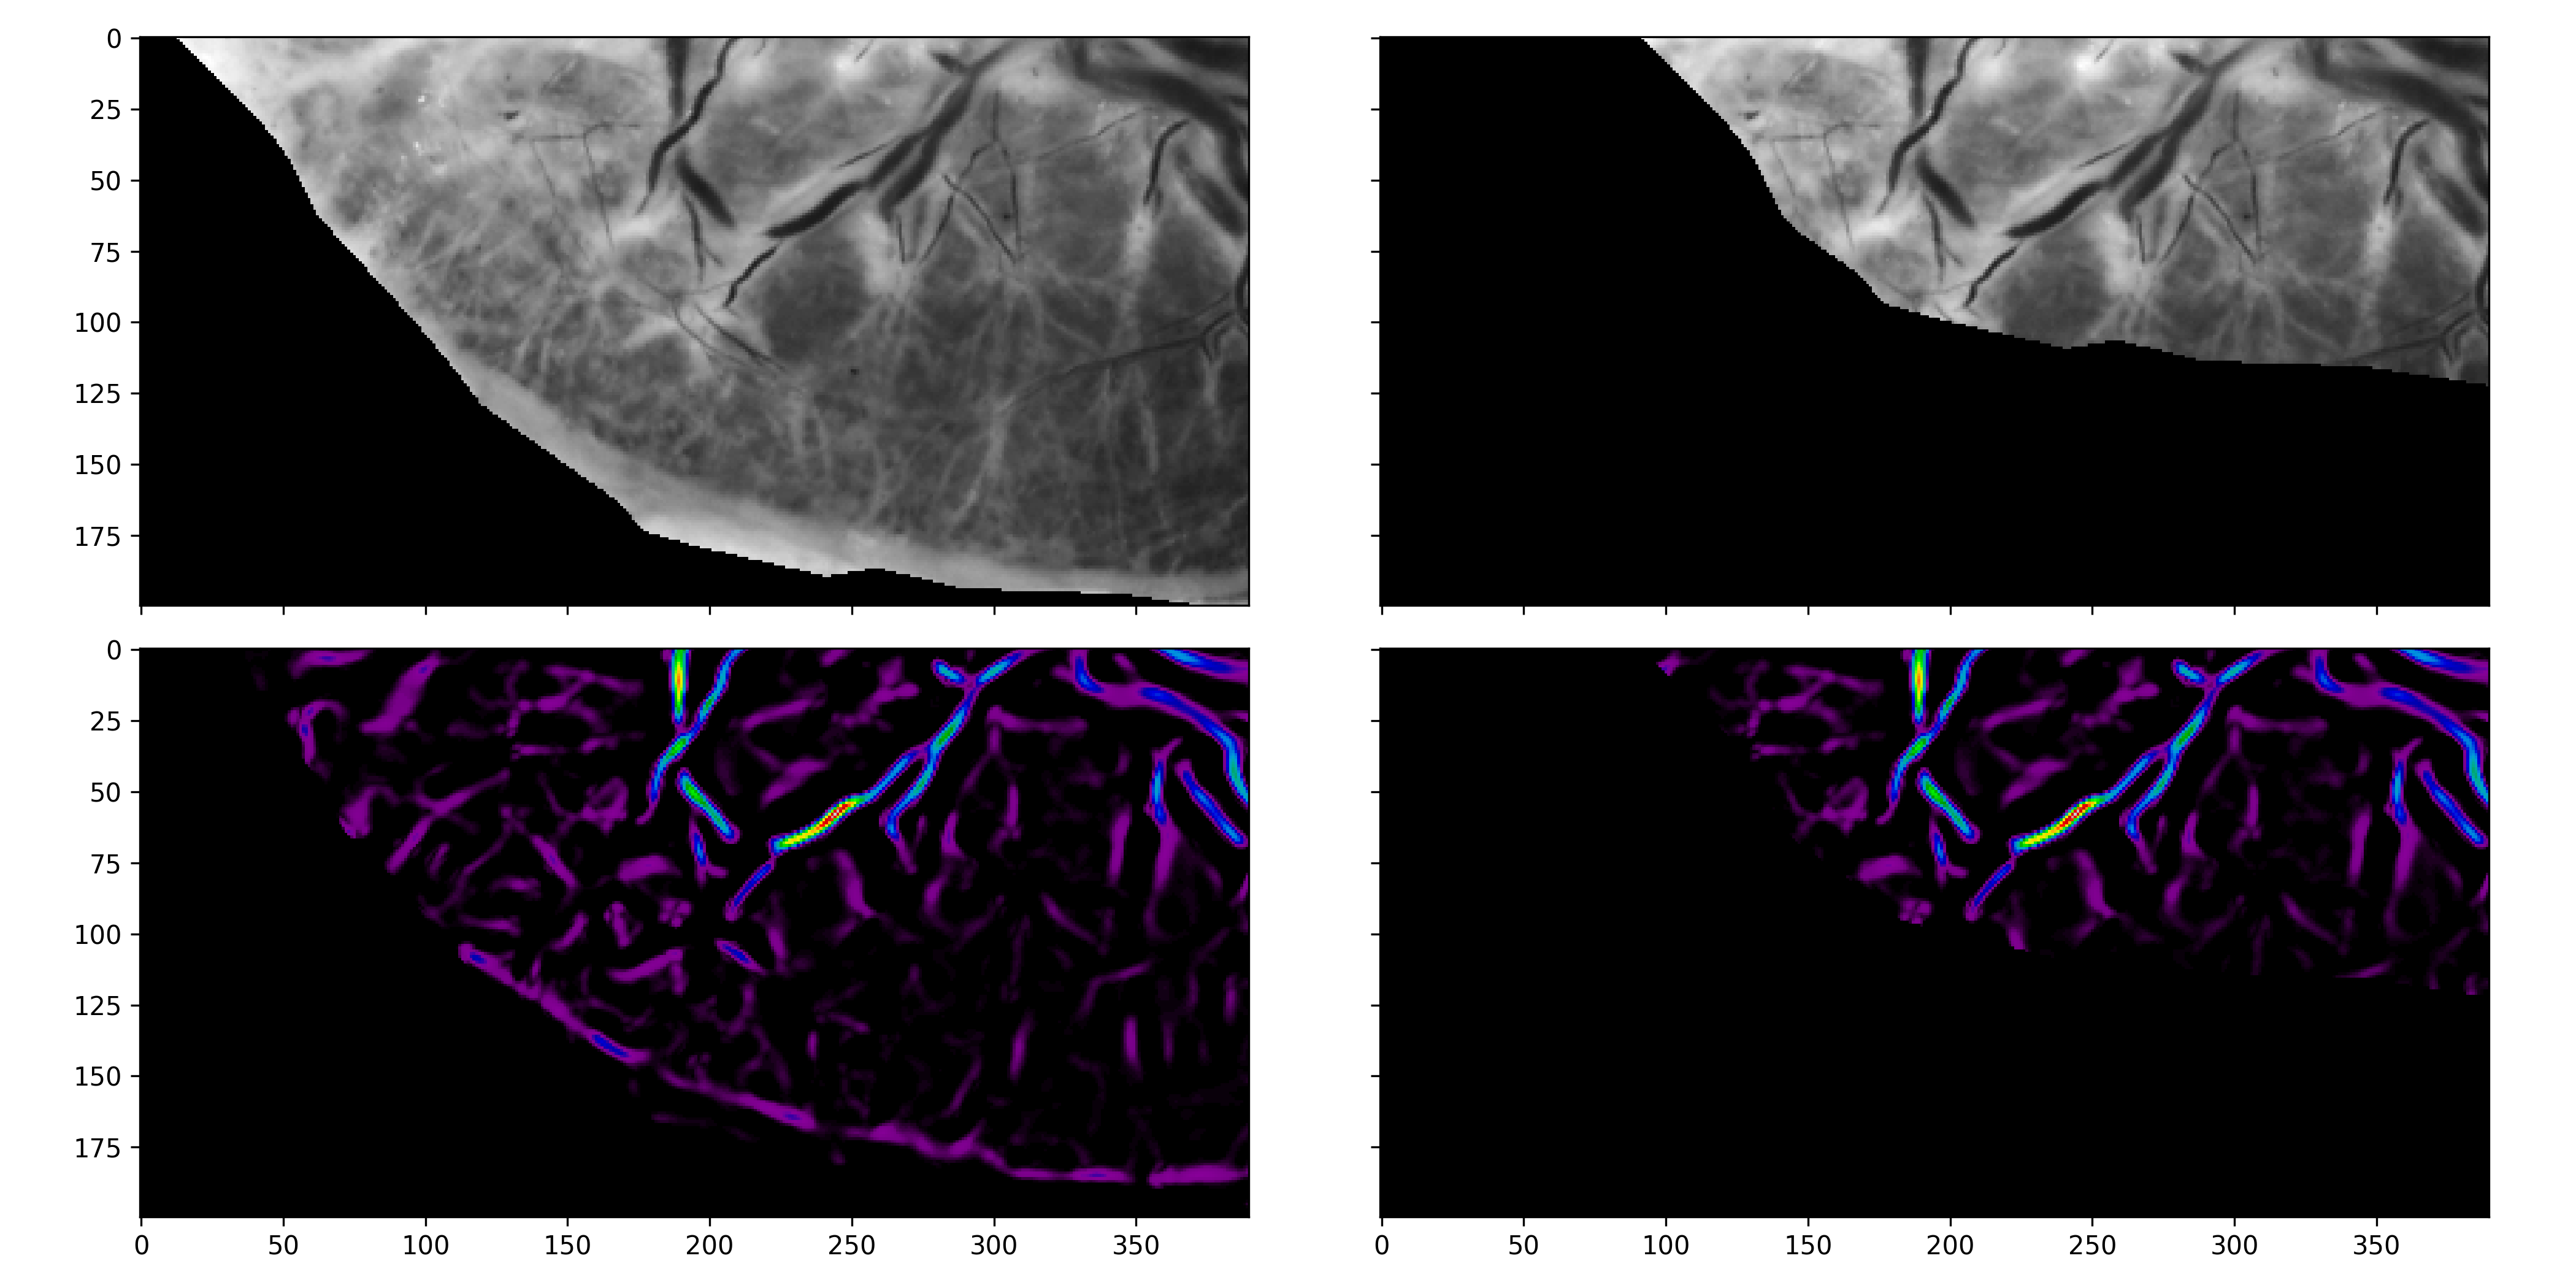
\includegraphics[width=\textwidth]{boundary_dilation_demo}
		\caption{Demonstration of boundary dilation}
	\end{figure}
	
	\ref{fig:boundary-demo} doesn't really show what I want it to, but this is what it would look like. Repeat with a smaller border. Maybe the issue doesn't occur with these as much? 	In the image above, $\sigma=3$ and border radius is 80 and all it does is get 	rid of the stupid natural boundary, not a weird frangi response. Which is important in itself, but I was having an error just between the edge of the image.
	
	The code for the above can by found by running \texttt{plate\_morphology.py} as a top-level script (that is, within the ``\texttt{if \_\_name\_\_ == \_\_main\_\_}'' block of the file).
	
\section{Multiscale Setup}

	Our multiscale Frangi filter requires a list of scales at which to probe. Each scale is chosen to accentuate features of a particular size, i.e. vessels of a particular radius. This  list of scales is denoted as $\Sigma := \{ \sigma_1, \sigma_2, \dots, \sigma_N\}$. 
	 
	The smallest one should be an effective size where details are expected to be found, and the largest should be an effective size as well. In fact, following \vtodo{CITE REF}, it is reasonable to select these logarithmically; that is,
	for some selected inputs $m < M$ we have
	
	\begin{equation}
	\sigma_1 = 2^{m} \; , \; \sigma_{j} = 2^{\left(m+\frac{M-m}{N-1}j\right)} \; , \; \sigma_N = 2^{M} \end{equation}
	
	That is, the exponents are spaced linearly from $m$ to $M$. This is achieved by the command
	\texttt{np.logspace(m,M,num=N)}. The idea is that the filter will respond better at its particular scale, but there are diminishing returns as $\sigma$ increases. While the filter's response may vary substantially between, say $\sigma=2$ and $\sigma=3$, there will be not be a substantial difference in response between, say, $\sigma=46$ and $\sigma=47$. There was an earlier benefit as well, that is still worth mentioning for historical reasons. Previously, computing the vesselness measure was very expensive, and thus it was simply not feasible to collect so many large scale readings. This is moot with the development of FFT-based Frangi filter.
	
	If there is no particular care taken in selecting a minimum and maximum range at which to probe, then we should assure that there is no noise being introduced at either ends, especially if the Frangi filter at which   ``throw out'' bad ones somehow. We will approach this issue in our discussion of ``variable thresholding'' see section \vtodo{add ref}.
	
	
	
	
	
	Convolve this via fft transform to get $L_{\sigma_i}$
	

\section{Applying Vesselness Measure}
Calculate the Hessian matrix of  and then the eigenvalues using the function \texttt{hfft.fft\_hessian}.

\vtodo{Show at this point or move elsewhere how features of  size $\sigma$ are isolated in this step at the appropriate scale.}

\begin{figure}
	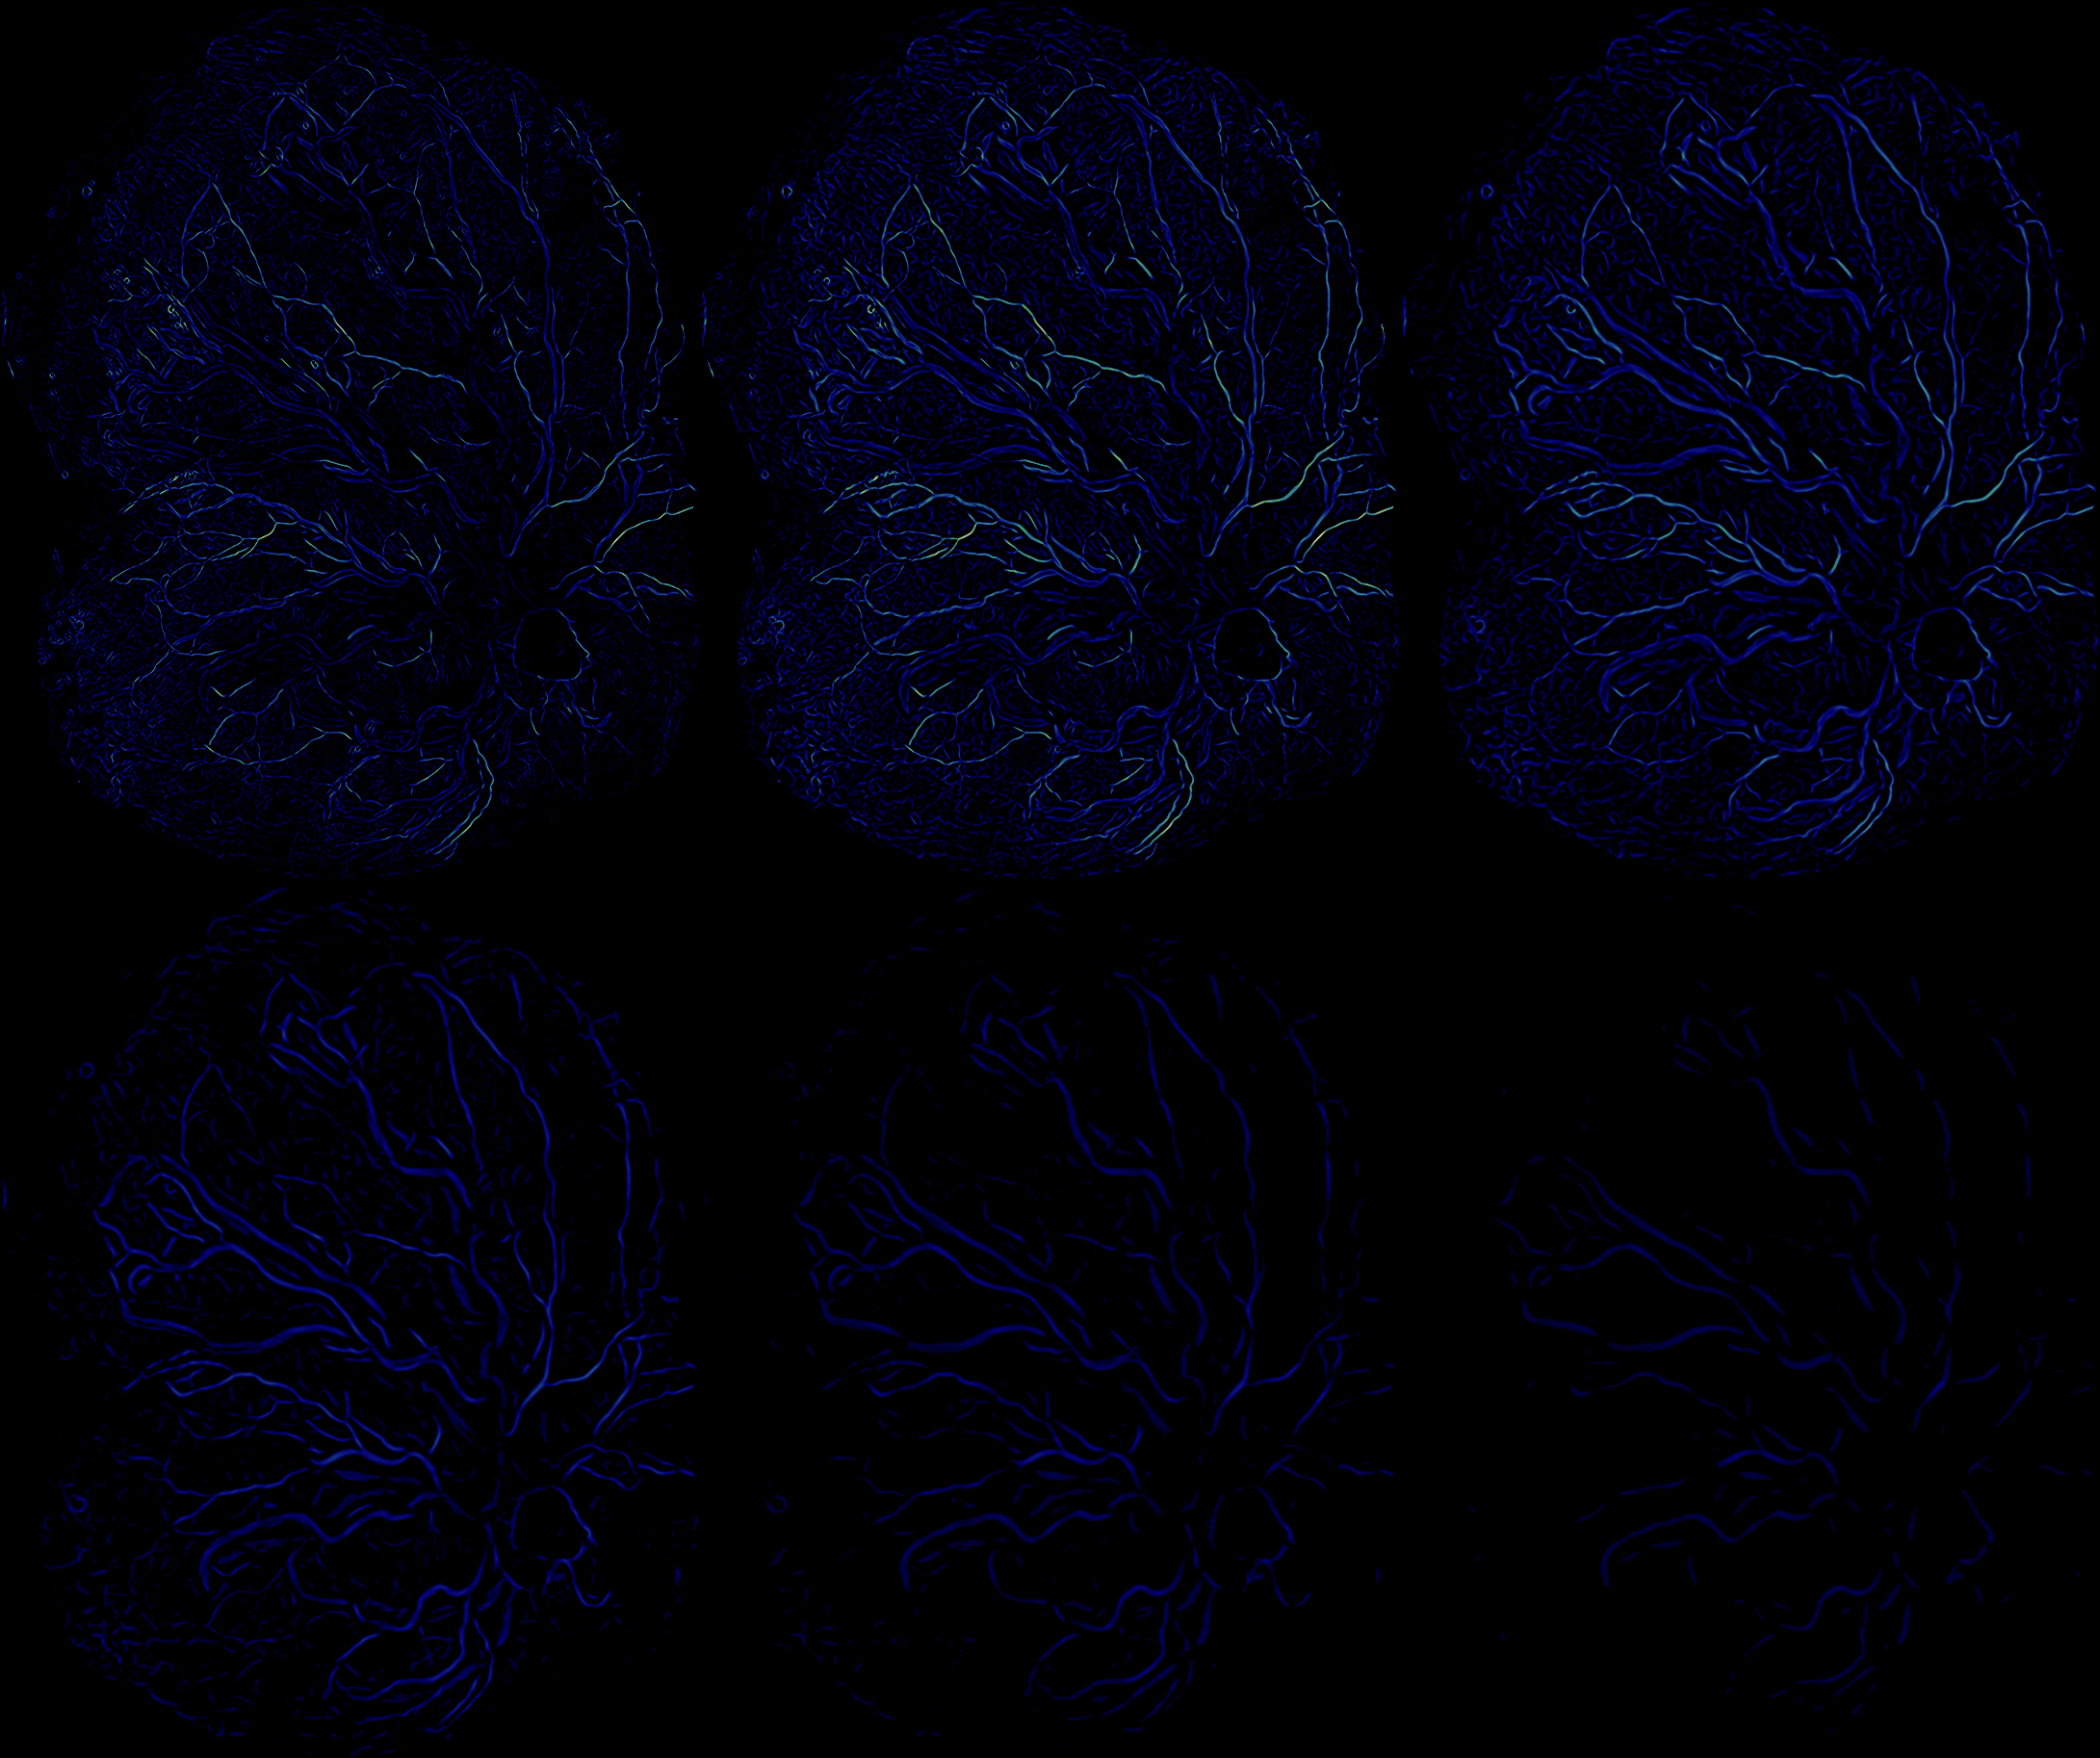
\includegraphics[width=\textwidth]{sweep_stitched_plate}
	\caption{Frangi vesselness score at several scales}
\end{figure}
\begin{figure}
	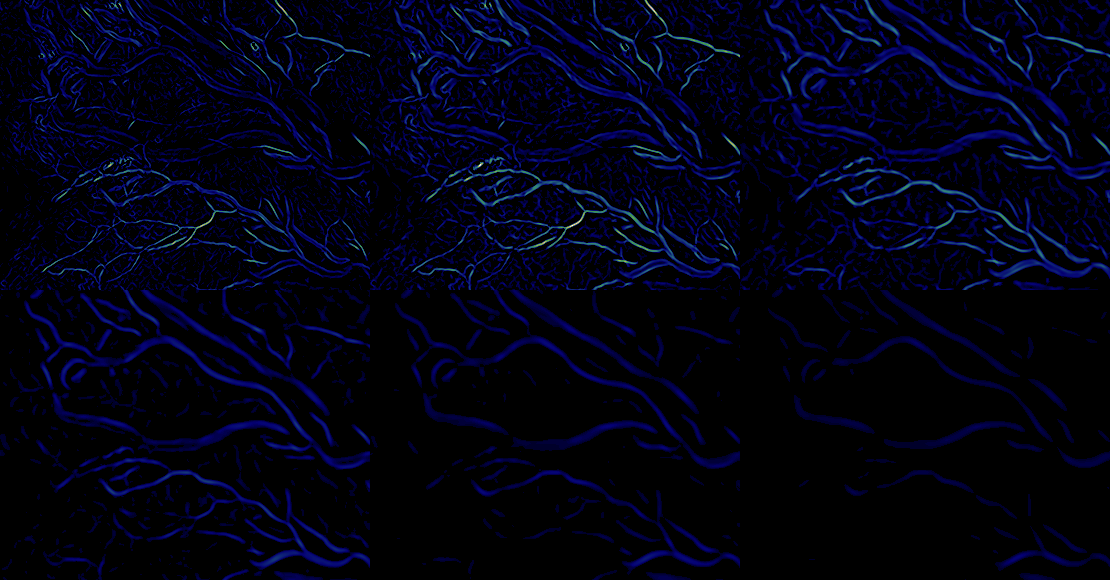
\includegraphics[width=\textwidth]{sweep_stitched_inset}
	\caption{Frangi vesselness score at several scales (inset)}
\end{figure}
\section{Scale-space post-processing}
\section{Multiscale Merging}
\section{Cleanup/Postprocessing}
\section{Measurements}

\section{NOTE DUMP}
	\vcomment{this is just a place to put commentary to sort/ rewrite later}
	
	\subsection{Erode plate / dilate boundary}
	
	Our function considers the placenta as a nonzero surface but the surface outside is zero (or, in many situations, masked). We're currently not implementing any way to ``reflect'' along the border, so instead the second degree behavior of the surface there will be incorrect in an area proportional to the scale size.
	
	Describe how that function works. Earlier efforts are wrong, whatever.
	
	The are which is affected should be larger than just the standard dropoff the gaussian however, since we're interested
	in second derivative information.
	
\section{Code Listings}
\vtodo{this goes in the appendix}